
%%%%%%%%%%%%%%%%%%%%%%%%%%%%%%%%%%%%%%%%%%%%%%%%%%%%%%%%%%%%%%%%%%%%%%%%
%Para las ecuaciones siempre es Ec.(n).
%Para las figuras siempre es Fig.n, incluso en el caption de la figura. Tambien las Tablas
%Para las referencias es [n]
%%%%%%%%%%%%%%%%%%%%%%%%%%%%%%%%%%%%%%%%%%%%%%%%%%%%%%%%%%%%%%%%%%%%%%%%

\documentclass[
reprint,
%notitlepage,
%superscriptaddress,
%groupedaddress,
%unsortedaddress,
%runinaddress,
%frontmatterverbose, 
%preprint,
%showpacs,preprintnumbers,
%nofootinbib,
%nobibnotes,
%bibnotes,
%11 pt,
amsmath,
amssymb,
aps,
pra,
%prb,
%rmp,
%tightenlines %esto hizo el milagro de sacar los espacios en blancos estocásticos (?)
 %prstab,
%prstper,
%floatfix,\textbf{}
]{revtex4-1} %Instalar primero para usarlo. Paquete malo.

%\documentclass[onecolumn, aps, amsmath,amssymb ]{article}
\usepackage{lipsum}  
\usepackage{graphicx}% Include figure files
\usepackage{subfig}
\usepackage{braket}
\usepackage{comment} %comment large chunks of text
\usepackage{dcolumn}% Align table columns on decimal point
\usepackage{bm}% bold math
%\usepackage{hyperref}% add hypertext capabilities
\usepackage[mathlines]{lineno}% Enable numbering of text and display math
%\linenumbers\relax % Commence numbering lines
\usepackage{mathtools} %% Para el supraíndice

\usepackage[nice]{nicefrac}

%%%%%%%El Señor Español%%%%%%%%%%%%%%%%%%%%%%%%%%%
\usepackage[utf8]{inputenc} %acento
\usepackage[
spanish, %El lenguaje.
es-tabla, %La tabla y no cuadro.
activeacute, %El acento.
es-nodecimaldot %Punto y no coma con separador de números
]{babel}
\usepackage{microtype} %para hacerlo más bonito :33 como vos (?) 
%%%%%%%%%%%%%%%%%%%%%%%%%%%%%%%%%%%%%%%%%%%%%%%%%%%
%%%%%%%%% Para que las imágenes se queden dónde las quiero (?
\usepackage{float}
%%%%%%%%%%

%%%%%%%%Cambia a Fig de Figure%%%%%%%%%%
\makeatletter
\renewcommand{\fnum@figure}{Fig. \thefigure} 
\makeatother
%%%%%%%%%%%%%%%%%%%%%%%%%%%%%%%%%%%%%%%%
\raggedbottom


\begin{document}
%%%%%%%%%%%%%%%%%%%%%%%%%%%%%%%%%%Título%%%%%%%%%%%%%%%%%%%%%%%%%%%%%%%%%%%%%%
%%%%%%%%%%%%%%%%%%%%%%%%%%%%%%%%%%%%%%%%%%%%%%%%%%%%%%%%%%%%%%%%%%%%%%%%%%%%%%

\title{Práctica 4: Aprendizaje supervisado en redes multicapa}
\author{Evelyn~G.~Coronel}

\affiliation{
Redes Neuronales - Instituto Balseiro}

\date[]{\lowercase{\today}} %%lw para lw, [] sin date

\begin{abstract}
En esta práctica se realiza el aprendizaje supervisado para distintas arquitecturas y problemas usando el algoritmo de backpropagation.
\end{abstract} 
\maketitle
%%%%%%%%%%%%%%%%%%%%%%%%%%%%%%%%%%%%%%%%%%%%%%%%%%%%%%%%%%%%%%%%%%%%%%%%%%%%%%%%%%%
% Podemos usar cualquiera de los dos comandos: \input o \include para incluir el texto
%\input{./Capitulo1/cap1.tex}

\section*{Ejercicio 1: XOR}

\subsection*{Casos base para el entrenamiento}

Para este problema básico, usamos todos los casos posibles para el entrenamiento, es decir, no tenemos ejemplos para testear la red neuronal. Estos casos se presentan en la Tabla\,\ref{tab:xor}.

\begin{table}[H]
\centering
\begin{tabular}{r | r | r}
Entrada 1 & Entrada 2 & Salida 	\\ \hline
-1 		  &-1	& +1 \\
-1 		  &+1	& -1\\
-1 		  &-1	& -1\\
+1 		  &+1	& +1\\
\end{tabular}
\caption{Todos los casos posibles para la función XOR.} \label{tab:xor}
\end{table}

Se utilizaron dos arquitecturas para el algoritmos de backpropagation, además de agregar una neurona extra para simular el bias. La función de transferencia para la salida fue $\tanh({x})$.

\subsection*{Arquitectura 2-2-1}

Un esquema de la arquitectura utilizada en este caso se muestra en la Fig.\,\ref{fig:arq-221}. En la misma se observa dos entradas, una capa oculta con 2 neuronas conectadas a cada entrada, y una salida conectada a la capa oculta.
\begin{figure}[H]
	\centering
	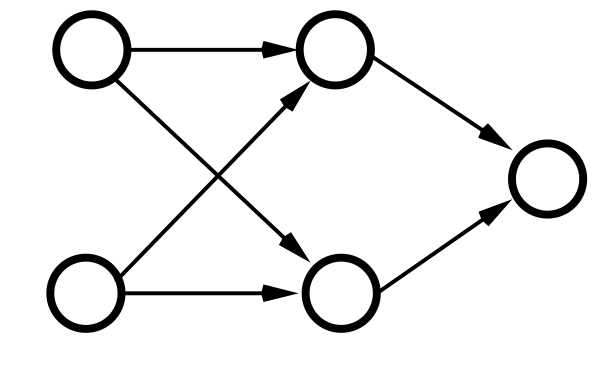
\includegraphics[width=0.35\textwidth]{ejer_1_221.png}
	\caption{Arquitectura 2-2-1}
	\label{fig:arq-221}
\end{figure}

\subsubsection*{Error en función de la época}

La función error utilizada en este caso  fue 

\subsection*{Arquitectura 2-1-1}


\begin{figure}[H]
	\centering
	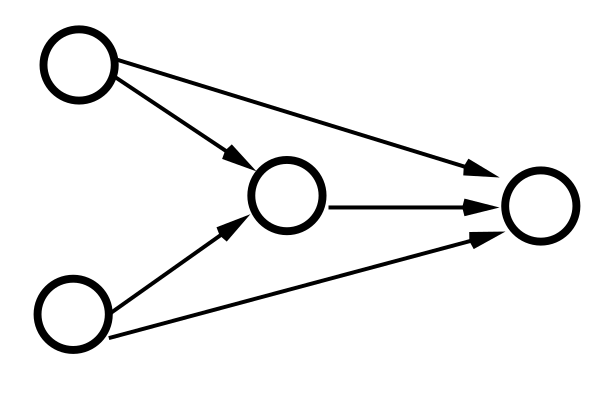
\includegraphics[width=0.35\textwidth]{ejer_1_211.png}
	\caption{Arquitectura 2-1-1}
	\label{fig:arq-211}
\end{figure}
\subsubsection*{Error en función de la época}

\section*{Ejercicio 2: XOR generalizado}

A diferencia del ejercicio anterior del XOR, ahora la función tiene N entradas, N$'$ neuronas en la capa oculta conectadas a las entradas, y una salida conectadas a todas las neuronas de la capa oculta. Esta arquitectura se muestra en la Fig.\,\ref{fig:arq-NN1}. La salida es $+1$ si el producto de las N entradas es $+1$ y $-1$ si el producto de las entradas es $-1.$

\begin{figure}[H]
	\centering
	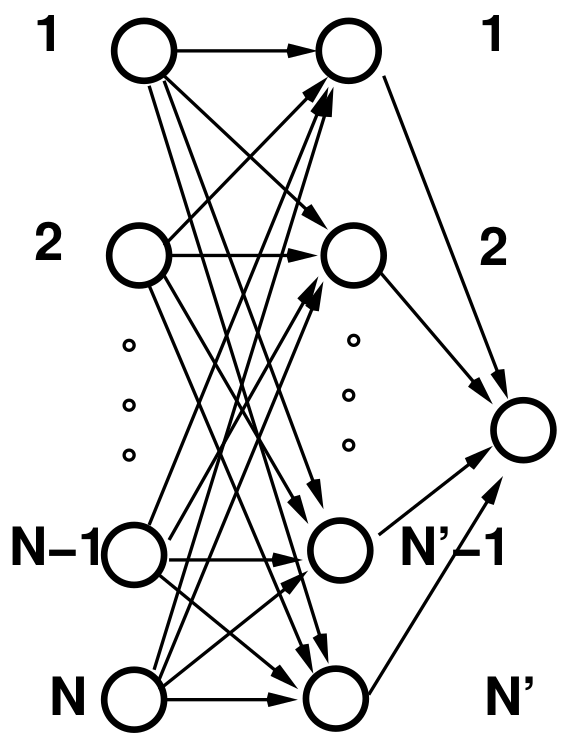
\includegraphics[width=0.35\textwidth]{ejer_2_NN1.png}
	\caption{Arquitectura N- N$'$ -1}
	\label{fig:arq-NN1}
\end{figure}

\subsection*{Entrenamiento}

\subsection*{Error en función de la época}

\section*{Ejercicio 3: Mapeo Logístico }

La función que la red neuronal busca solución es conocida, que la función logística, dada por la Ec.\,\ref{eq:logistica} del tipo 
\begin{equation}
	x(t+1) = 4x(t)(1+x(t))
	\label{eq:logistica}
\end{equation}

\begin{figure}[H]
	\centering
	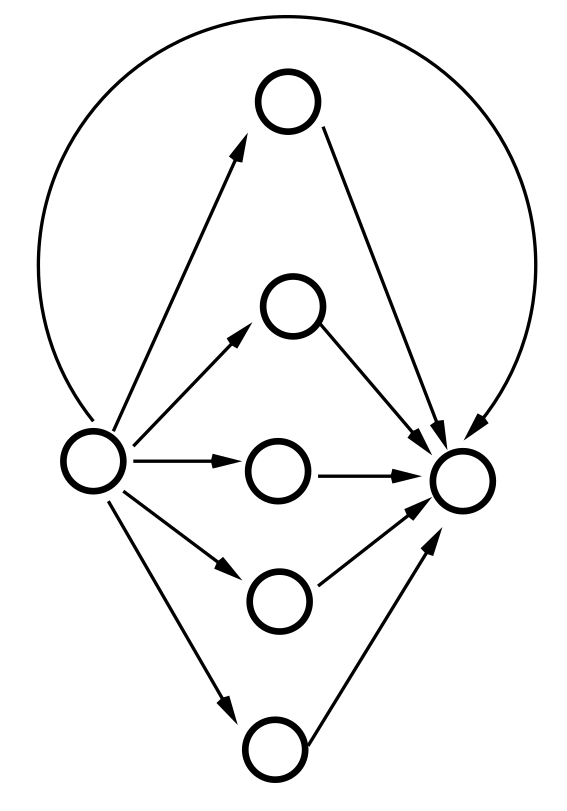
\includegraphics[width=0.3\textwidth]{ejer_3.png}
	\caption{Arquitectura para solucionar el mapeo logístico.}
	\label{fig:arq-mapeo}
\end{figure}

\subsection*{Entrenamiento}

\subsection*{Error en función de la época}



\end{document}